\section{Copia por defecto}

\begin{frame}[fragile]{Operaciones de copia generadas}
\begin{itemize}
  \item Por cada tipo definido por el usuario se generan 
        de \textmark{forma automática} \textgood{dos operaciones de copia}:
    \begin{itemize}

      \mode<presentation>{\vfill\pause}
      \item \textgood{Construcción de copia}.
\begin{lstlisting}
T y;
T x{y};  // Construcción de copia. Iniciación directa.
T x = y; // Construcción de copia. Iniciación de copia.
\end{lstlisting}

      \mode<presentation>{\vfill\pause}
      \item \textgood{Asignación de copia}.
\begin{lstlisting}
T x, y;
x = y; // Asignación de copia
\end{lstlisting}
    \end{itemize}

  \mode<presentation>{\vfill\pause}
  \item Implementación por defecto:
    \begin{itemize}
      \item Invocación (recursiva) de \textgood{operaciones de copia} 
            \textmark{para cada miembro}.
      \item La copia de \textmark{miembros tipos primitivos} es la 
            \textgood{copia del valor}.
    \end{itemize}
\end{itemize}
\end{frame}

\mode<presentation>{
\begin{frame}[t]{Vector numérico}
\begin{block}{vecnum.hpp}
\lstinputlisting[lastline=14]{ejemplos/03-copia/vecnum-nocopy/vecnum.hpp}
\ldots
\end{block}
\end{frame}

\begin{frame}[t]{Vector numérico}
\begin{block}{vecnum.hpp}
\ldots
\lstinputlisting[firstline=16]{ejemplos/03-copia/vecnum-nocopy/vecnum.hpp}
\end{block}
\end{frame}
}

\mode<article>{
\begin{frame}[t,fragile]{Vector numérico}
\begin{block}{vecnum.hpp}
\lstinputlisting{ejemplos/03-copia/vecnum-nocopy/vecnum.hpp}
\end{block}
\end{frame}
}

\begin{frame}[t,fragile]{Implementación de vector numérico}
\begin{block}{vecnum.cpp}
\lstinputlisting{ejemplos/03-copia/vecnum-nocopy/vecnum.cpp}
\end{block}
\end{frame}

\begin{frame}[t, fragile]{Usando \textbf{vecnum}}
\begin{columns}[T]

\column{.5\textwidth}
\begin{block}{main.cpp}
\lstinputlisting{ejemplos/03-copia/vecnum-nocopy/main.cpp}
\end{block}

\pause
\column{.5\textwidth}
\begin{itemize}
\item Resultado de ejecución:
\end{itemize}
\begin{lstlisting}[style=terminal]
v1: (0, 0, 5, 0, 3.5)
v2: (0, 0, 5, 0, 3.5)
free(): double free detected in tcache 2
Abortado (`core' generado)
\end{lstlisting}
\begin{itemize}
\item \textbad{Problema}: Doble liberación de memoria.
\end{itemize}
\end{columns}

\end{frame}

\begin{frame}[fragile]
\begin{lstlisting}[style=terminal,basicstyle=\tiny\ttfamily]
$ valgrind ./vecnum_nocopy 
\end{lstlisting}
\begin{lstlisting}[style=terminal,basicstyle=\tiny\ttfamily]
==2710003== Memcheck, a memory error detector
==2710003== Copyright (C) 2002-2017, and GNU GPL'd, by Julian Seward et al.
==2710003== Using Valgrind-3.15.0 and LibVEX; rerun with -h for copyright info
==2710003== Command: ./vecnum_nocopy
==2710003== 
v1: (0, 0, 5, 0, 3.5)
v2: (0, 0, 5, 0, 3.5)
==2710003== Invalid free() / delete / delete[] / realloc()
==2710003==    at 0x483D74F: operator delete[](void*) (in /usr/lib/x86_64-linux-gnu/valgrind/vgpreload_memcheck-amd64-linux.so)
==2710003==    by 0x1094BA: vecnum::~vecnum() (vecnum.hpp:12)
==2710003==    by 0x109364: main (main.cpp:6)
==2710003==  Address 0x4dffc80 is 0 bytes inside a block of size 40 free'd
==2710003==    at 0x483D74F: operator delete[](void*) (in /usr/lib/x86_64-linux-gnu/valgrind/vgpreload_memcheck-amd64-linux.so)
==2710003==    by 0x1094BA: vecnum::~vecnum() (vecnum.hpp:12)
==2710003==    by 0x109358: main (main.cpp:10)
==2710003==  Block was alloc'd at
==2710003==    at 0x483C583: operator new[](unsigned long) (in /usr/lib/x86_64-linux-gnu/valgrind/vgpreload_memcheck-amd64-linux.so)
==2710003==    by 0x109455: vecnum::vecnum(int) (vecnum.hpp:10)
==2710003==    by 0x109295: main (main.cpp:6)
==2710003== 
==2710003== 
==2710003== HEAP SUMMARY:
==2710003==     in use at exit: 0 bytes in 0 blocks
==2710003==   total heap usage: 3 allocs, 4 frees, 73,768 bytes allocated
...
$
\end{lstlisting}
\end{frame}

\begin{frame}[t,fragile]{Analizando resultado de valgrind}
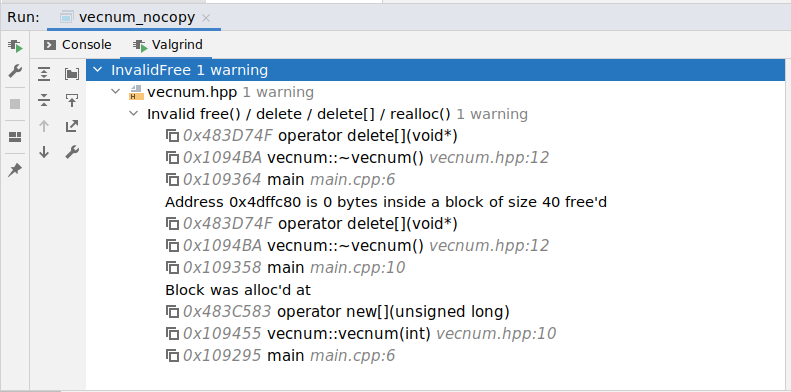
\includegraphics[width=\textwidth]{images/03-copia/vecnum-nocopy-valgrind.png}
\end{frame}

\begin{frame}[t,fragile]{Copia y liberación}
\begin{itemize}
  \item \textbad{Problema}: Al realizar la copia, se ha copiado la dirección del array.
    \begin{itemize}
      \item Los dos vectores están compartiendo el mismo array.
      \item Se está desasignando dos veces un mismo bloque de memoria.
    \end{itemize}
\end{itemize}

\mode<presentation>{\vfill}
\begin{tikzpicture}
\tikzset{
    bloque/.style={rectangle,draw=black, top color=white, bottom color=blue!50,
                   very thick, inner sep=0.5em, minimum size=0.6cm, text centered, font=\tiny},
    flecha/.style={->, >=latex', shorten >=1pt, thick},
    etiqueta/.style={text centered, font=\tiny} 
}  
\node[bloque] (bsize) {5};
\node[bloque,right=0cm of bsize] (bptr) { };
\node[bloque,right=0.5cm of bptr] (v0) {0.0};
\node[bloque,right=0cm of v0] (v1) {0.0};
\node[bloque,right=0cm of v1] (v2) {5.0};
\node[bloque,right=0cm of v2] (v3) {0.0};
\node[bloque,right=0cm of v3] (v4) {3.5};
\draw[flecha] (bptr) -- (v0);
\node[etiqueta, left=0.1cm of bsize] {v1:};
\node[etiqueta, above=0cm of bsize] {tam};

\node[bloque, below=1cm of bsize] (bsize2) {5};
\node[bloque,right=0cm of bsize2] (bptr2) { };
\draw[flecha] (bptr2) -- (v0);
\node[etiqueta, left=0.1cm of bsize2] {v2:};

\end{tikzpicture}
\end{frame}
